
\documentclass[journal=tosc,final]{iacrtrans}
\begin{document}
\section{Initial Challenges}


% \begin{table}
%     \centering
%     \begin{tabular}{|c|c|} \hline 
%          3-5& 4\\ \hline 
%          6-13& 5\\ \hline 
%          14-27& 6\\ \hline 
%          28-59& 7\\ \hline 
%          60-119& 8\\ \hline 
%          120-247& 9\\ \hline 
%          248-495& 10\\ \hline 
%          496-1007&	11\\ \hline 
%          1008-2031&	12 \\ \hline
%     \end{tabular}
%     \caption{Polynomial degrees to multiplicative depths}
%     \label{tab:my_label}
% \end{table}

\subsection{Logistic Function Challenge}
The logistic (a.k.a., sigmoid) function forms the basis for logistic regression-based machine learning. Additionally, it is commonly employed as a non-linear activation function in neural networks. In homomorphic contexts like CKKS, which only support polynomial arithmetic operations, expressing the sigmoid function as a polynomial is not feasible. Consequently, various series, such as the Taylor series or the Chebyshev series, are utilized to approximate the sigmoid function. Recent efforts have focused on developing privacy-preserving models for logistic regression training and inference by employing similar approximations of the logistic function~\cite{lr1,lr2,lr3,lr4}. Therefore, it is crucial to investigate the extent to which we can approximate the logistic function under constrained multiplicative depth. 

To address this, the challenge was structured with two sets of test cases, distinguished solely in terms of the permitted multiplicative depth. The input values for both sets of test cases are confined to the range of $[-25, 25]$. The straightforward logistic evaluation of this range is illustrated in Figure~\ref{fig:sigmoid_approx_cheb}. As previously mentioned, one common method for approximating the logistic function involves employing the Chebyshev series. However, the Chebyshev series provides results only for values within the range $[-1,1]$. Consequently, to apply the Chebyshev series to broader ranges (e.g., $[a,b]$), the input polynomial (e.g., $x$) is scaled to bring it to the interval $[-1,1]$ as outlined below, ensuring the effectiveness of the Chebyshev approximation.
\begin{align}
    x' & = \frac{2x - (b+a)}{b-a}
\end{align}
    $ \text{when, } |a|=|b|, a \neq b, \text{ and } \omega=\frac{b-a}{2} $
\begin{align}
    x' & =  \frac{x}{\omega}
\end{align}
The scaled ciphertext $x'$ is subsequently employed for the approximation. However, note that this scaling results in the loss of one multiplicative depth. This aspect is explicitly mentioned in the \href{https://github.com/openfheorg/openfhe-development/blob/main/src/pke/examples/FUNCTION_EVALUATION.md}{library documentation} for function evaluation. A similar proposal is also made in prior works in the literature~\cite{Sign_approx_comp_poly}, where solutions for the interval $[-1,1]$ are proposed, along with suggestions for scaling to accommodate larger intervals.

\begin{figure}[t]
    \begin{minipage}{.48\textwidth}
    \centering
    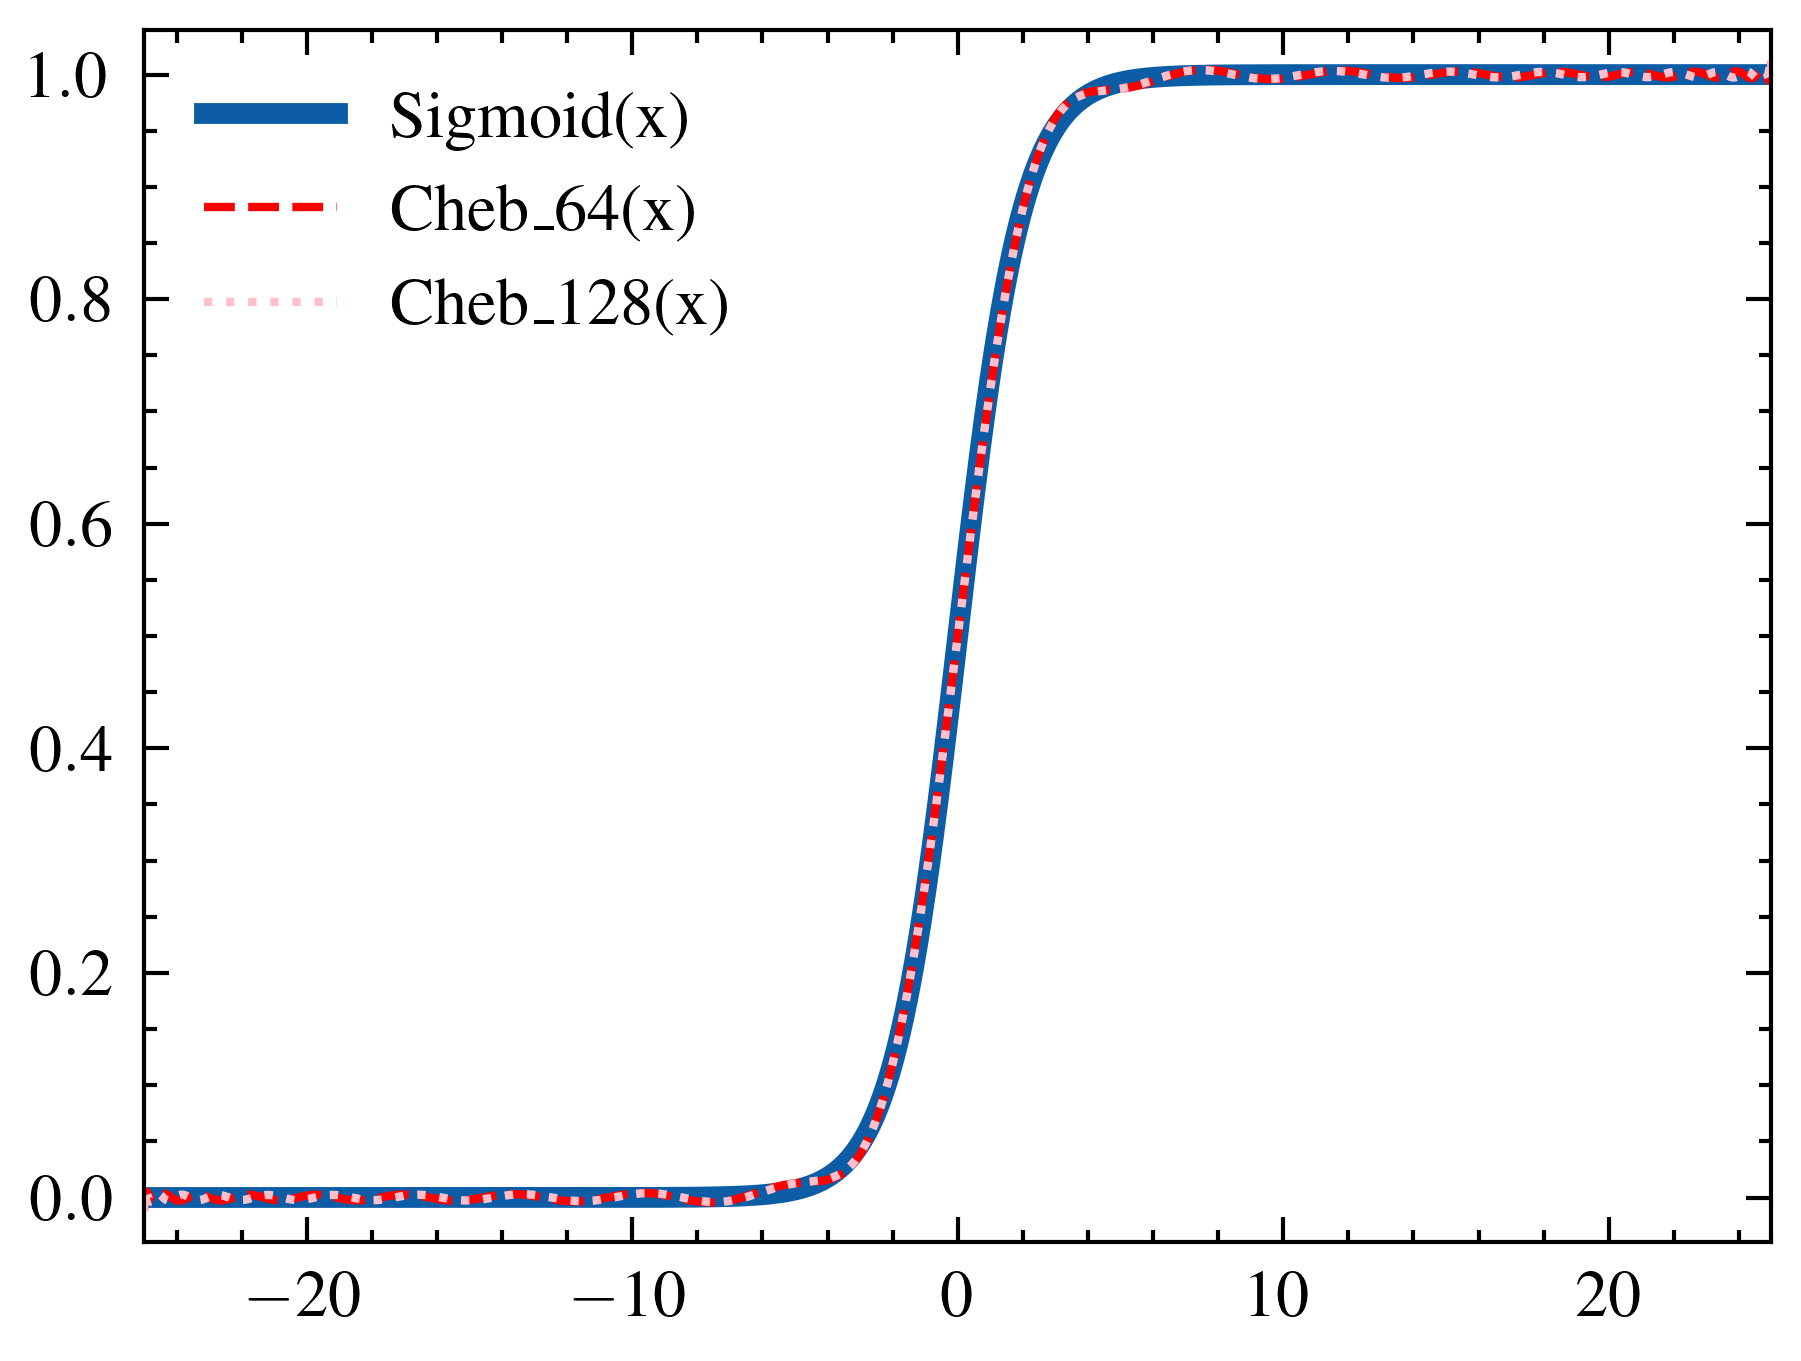
\includegraphics[width=\textwidth]{iacrtrans-0.93/figures/sigmoid_2.png}
    \captionof{\textbf{a)} }{Sigmoid and its function approximation using Chebyshev series (64,128).}
    \end{minipage}
    \hfill
    \begin{minipage}{.48\textwidth}
    \centering
    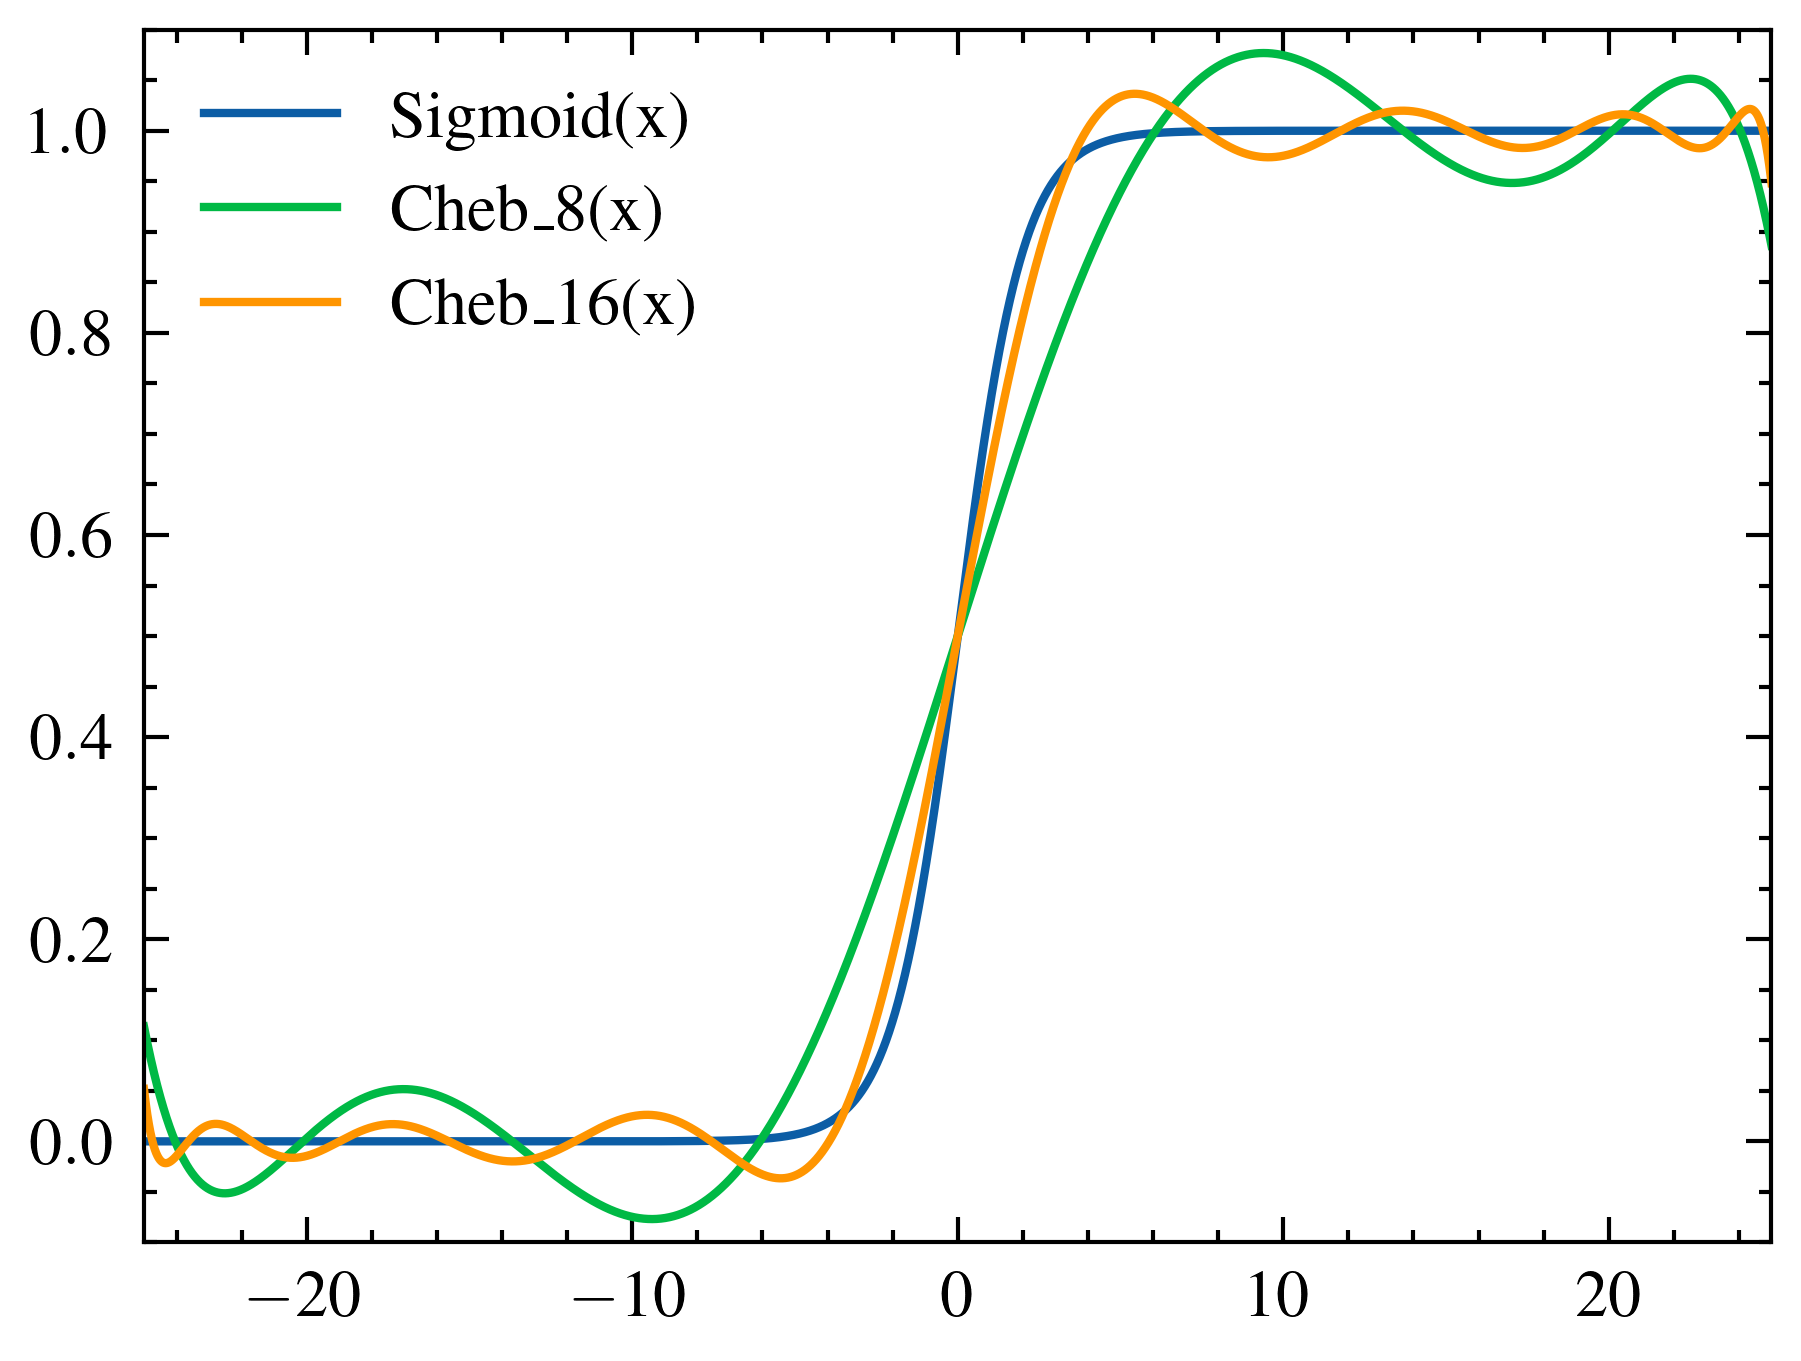
\includegraphics[width=\textwidth]{iacrtrans-0.93/figures/sigmoid_1.png}
    \captionof{\textbf{b)} }{Sigmoid and its function approximation using Chebyshev series (8,16).}
    \end{minipage}
    \caption{Function approximations for the sigmoid function.}
    \label{fig:sigmoid_approx_cheb}
\end{figure}

Consequently, when presented with a challenge specifying a multiplicative depth $d$ over an arbitrary range $[a,b],\text{ such that } a\neq-1\text{ and }b\neq1 $, the available Chebyshev series approximation technique allows us to evaluate up to a depth of $d-1$ at best. To fully exploit this using OpenFHE, the technique described in the SIGN challenge solution can be applied. However, it becomes evident that although reducing the depth from 7 to 6, as shown in Figure~\ref{fig:sigmoid_approx_cheb} (a) does not result in a significant loss of accuracy, but dropping from 4 to 3 entails a considerable loss (Figure~\ref{fig:sigmoid_approx_cheb} (b)). Therefore, our exploration focuses on enhancing this existing technique to yield the best approximation results.




%Our best approaches for the two test test cases are as follows:



 \subsubsection{The 1st Test case}
The first test case permits a multiplicative depth of seven. Initially, we assess the capabilities of the current implementation to determine how far we can go. Notably, with OpenFHE's ChebyshevPS implementation, we find that we can evaluate the Chebyshev series up to the coefficient 59. Through the application of the strategy employed in the SIGN challenge, this evaluation can be extended to 63 coefficients, resulting in an impressive accuracy of $99.99\%$. To walk the extra mile (or 0.01\%) for achieving complete accuracy, we delve into the recursive unroll of \textbf{T}$_{65}$ as outlined below:
 \begin{align}
    \text{c}\times\textbs{T}_{65} && \rightarrow && \text{2c}\times\textbs{T}_{32}\times\textbs{T}_{33}-\text{c}\times\textbs{T}_{1} && \rightarrow &&  \textbs{T}_{32}\times(\text{2c}\times\textbs{T}_{33})-\text{c}\times\textbs{T}_{1}\\
    \text{2c}\times\textbs{T}_{33} && \rightarrow &&  \text{4c}\times\textbs{T}_{16}\times\textbs{T}_{17}-\text{2c}\times\textbs{T}_{1} && \rightarrow  && \textbs{T}_{16}\times(\text{4c}\times\textbs{T}_{17})-\text{2c}\times\textbs{T}_{1}\\
    \text{4c}\times\textbs{T}_{17} && \rightarrow  && \text{8c}\times\textbs{T}_{8}\times\textbs{T}_{9}-\text{4c}\times\textbs{T}_{1} && \rightarrow &&  \textbs{T}_{8}\times(\text{8c}\times\textbs{T}_{9})-\text{4c}\times\textbs{T}_{1}\\
    \text{8c}\times\textbs{T}_{9} && \rightarrow &&  \text{16c}\times\textbs{T}_{4}\times\textbs{T}_{5}-\text{8c}\times\textbs{T}_{1} && \rightarrow &&  \textbs{T}_{4}\times(\text{16c}\times\textbs{T}_{5})-\text{8c}\times\textbs{T}_{1}\\
    \text{16c}\times\textbs{T}_{5} && \rightarrow &&  \text{32c}\times\textbs{T}_{2}\times\textbs{T}_{3}-\text{16c}\times\textbs{T}_{1} && \rightarrow &&  \textbs{T}_{2}\times(\text{32c}\times\textbs{T}_{3})-\text{16c}\times\textbs{T}_{1}
\end{align}
This recursive breakdown is just one of the numerous possible approaches. Examining this breakdown, we notice that at each step, the two coefficients to be multiplied are at different depths, and one consistently exceeds the permitted multiplicative depth at that level. Consequently, we continue the breakdown until we reach $\textbf{T}_2$ and $\textbf{T}_3$, which can be represented as follows:
 \begin{align}
    \textbs{T}_{2} && \rightarrow && \text{2x}'^2-1 && \text{\textcolor{gray}{// Multiplicative depth 2}}\\
    c\times\textbs{T}_{3} && \rightarrow && \text{4cx}'^3-\text{3cx}'  && \text{\textcolor{gray}{// Multiplicative depth 3}}
\end{align}
Note that $\textbf{T}_3$ is at a higher depth compared to $\textbf{T}_2$. The computation of $\textbf{T}_{65}$ relies on our ability to compute $32c\times\textbf{T}_3$ while remaining at the same multiplicative depth as $\textbf{T}_2$. In this context, we emphasize that 'the sky is not the limit' and indeed, there is a method to accomplish this, as illustrated in the equations below:
\begin{align}
     32c\times\textbs{T}_{3} && \rightarrow && \frac{128c}{\omega^3} x^3-\text{96cx}'  && \text{\textcolor{gray}{// Multiplicative depth 2}}\\
     32c\times\textbs{T}_{3} && \rightarrow && (\frac{128c}{\omega^3}x)(x^2)-\text{96cx}'  && \text{\textcolor{gray}{// Multiplicative depth 2}}
\end{align}

We want to emphasize that, similar to the case of the sign function, the logistic function is also an odd function. Consequently, only the odd coefficients of the Chebyshev series contribute to the approximation. Leveraging recursive breakdowns like the one for $\textbf{T}_{65}$, we calculate odd series coefficients up to $\textbf{T}_{77}$, successfully achieving our target of $100\%$ accuracy for this particular test case. While this approach sufficed for the current scenario, it remains intriguing to investigate how far we can extend this breakdown before reaching limitations. 
 
 \subsubsection{The 2nd Test case}
In this particular test case, a multiplicative depth of only four is mandated. The straightforward Chebyshev series computation up to coefficient seven resulted in an accuracy of $88.12$, falling short of the minimum requirement of 90\%. Therefore, a comprehensive exploration of the approach identified in the previous test case becomes necessary. It is important to highlight that Chebyshev series computation can be transformed into a simple polynomial evaluation. Given the low multiplicative depth, it becomes evident that converting the Chebyshev computation to polynomial evaluation is crucial for a thorough investigation of the limitations of the aforementioned technique.

The coefficients generated for evaluating an unscaled polynomial of degree 16 are as follows: \{0.5000000000005096, 0.1901080095983654, 0.0, -0.004141898216566491, 0.0, 4.836391763505995e-05, 0.0, -2.96844677821543e-07, 0.0, 1.0135652189233364e-09, 0.0, -1.937580840140624e-12, 0.0, 1.938529697379292e-15, 0.0, -7.898895000665899e-19, 0.0\}. Notably, the values of these coefficients exhibit a progressive decrease. This diminishing trend arises because the scaling factor, previously managed by the ciphertext, is now concentrated at the coefficient level. We compute the evaluation up to $x^7$ in a very straightforward manner, as shown below
\begin{align}
     \texttt{SUM}_7 = (c_7\times x^4)\times x^3 +(c_5\times x^3)\times x^2 +(c_3\times x^2)\times x + c_1\times x+ c_0 
\end{align}

For the next evaluation, it is apparent that coefficients 9, 11, 13, and 15 are exceedingly small, nearly reaching the limits of the scaling factor. There exists a potential for computational errors if not handled cautiously. Hence, we recommend breaking down the computation of higher coefficients into smaller chunks, as outlined below:

\begin{align}
    y_1 && = && (10^{-3}\times x )\times x && \text{\textcolor{gray}{$10^{-3}\times x^2$ at depth 2}}\\
    y_2 && = && (c_9\times 10^{6} \times x )\times x && \text{\textcolor{gray}{$c_9 \times 10^{6}\times x^2$ at depth 2}}\\
    c_9\times x^9 && = && (y_1\times y_1) \times (y_2\times x^3) &&
\end{align}

Applying this approach, we can extend the evaluation up to $x^{13}$ as depicted in the equation below. This limitation arises because the coefficient computation needs to be divided into at least two parts. The maximum degree achievable with two constant multiplications in this manner is $x^{14}$. Consequently, we have reached the limit of this technique. 
\begin{align}
    y_1 && = && (10^{-6}\times x )\times x^2 && \text{\textcolor{gray}{$10^{-6}\times x^3$ at depth 2}}\\
    y_2 && = && (c_{13}\times 10^{12} \times x )\times x^2 && \text{\textcolor{gray}{$c_{13} \times 10^{12}\times x^3$ at depth 2}}\\
    c_{13}\times x^{13} && = && (y_1\times y_1) \times (y_2\times x^4) &&
\end{align}

The additional computation up to $x^{13}$ led to an enhancement in accuracy from $88.12\%$ to $96.6\%$. This is a significant improvement in the attainable accuracy, and exploring the effectiveness of this technique in approximating functions other than logistic functions at different depths would be an interesting avenue for future exploration.

  
\subsection{SIGN Challenge}
\begin{figure}
    \begin{minipage}{.48\textwidth}
    \centering
    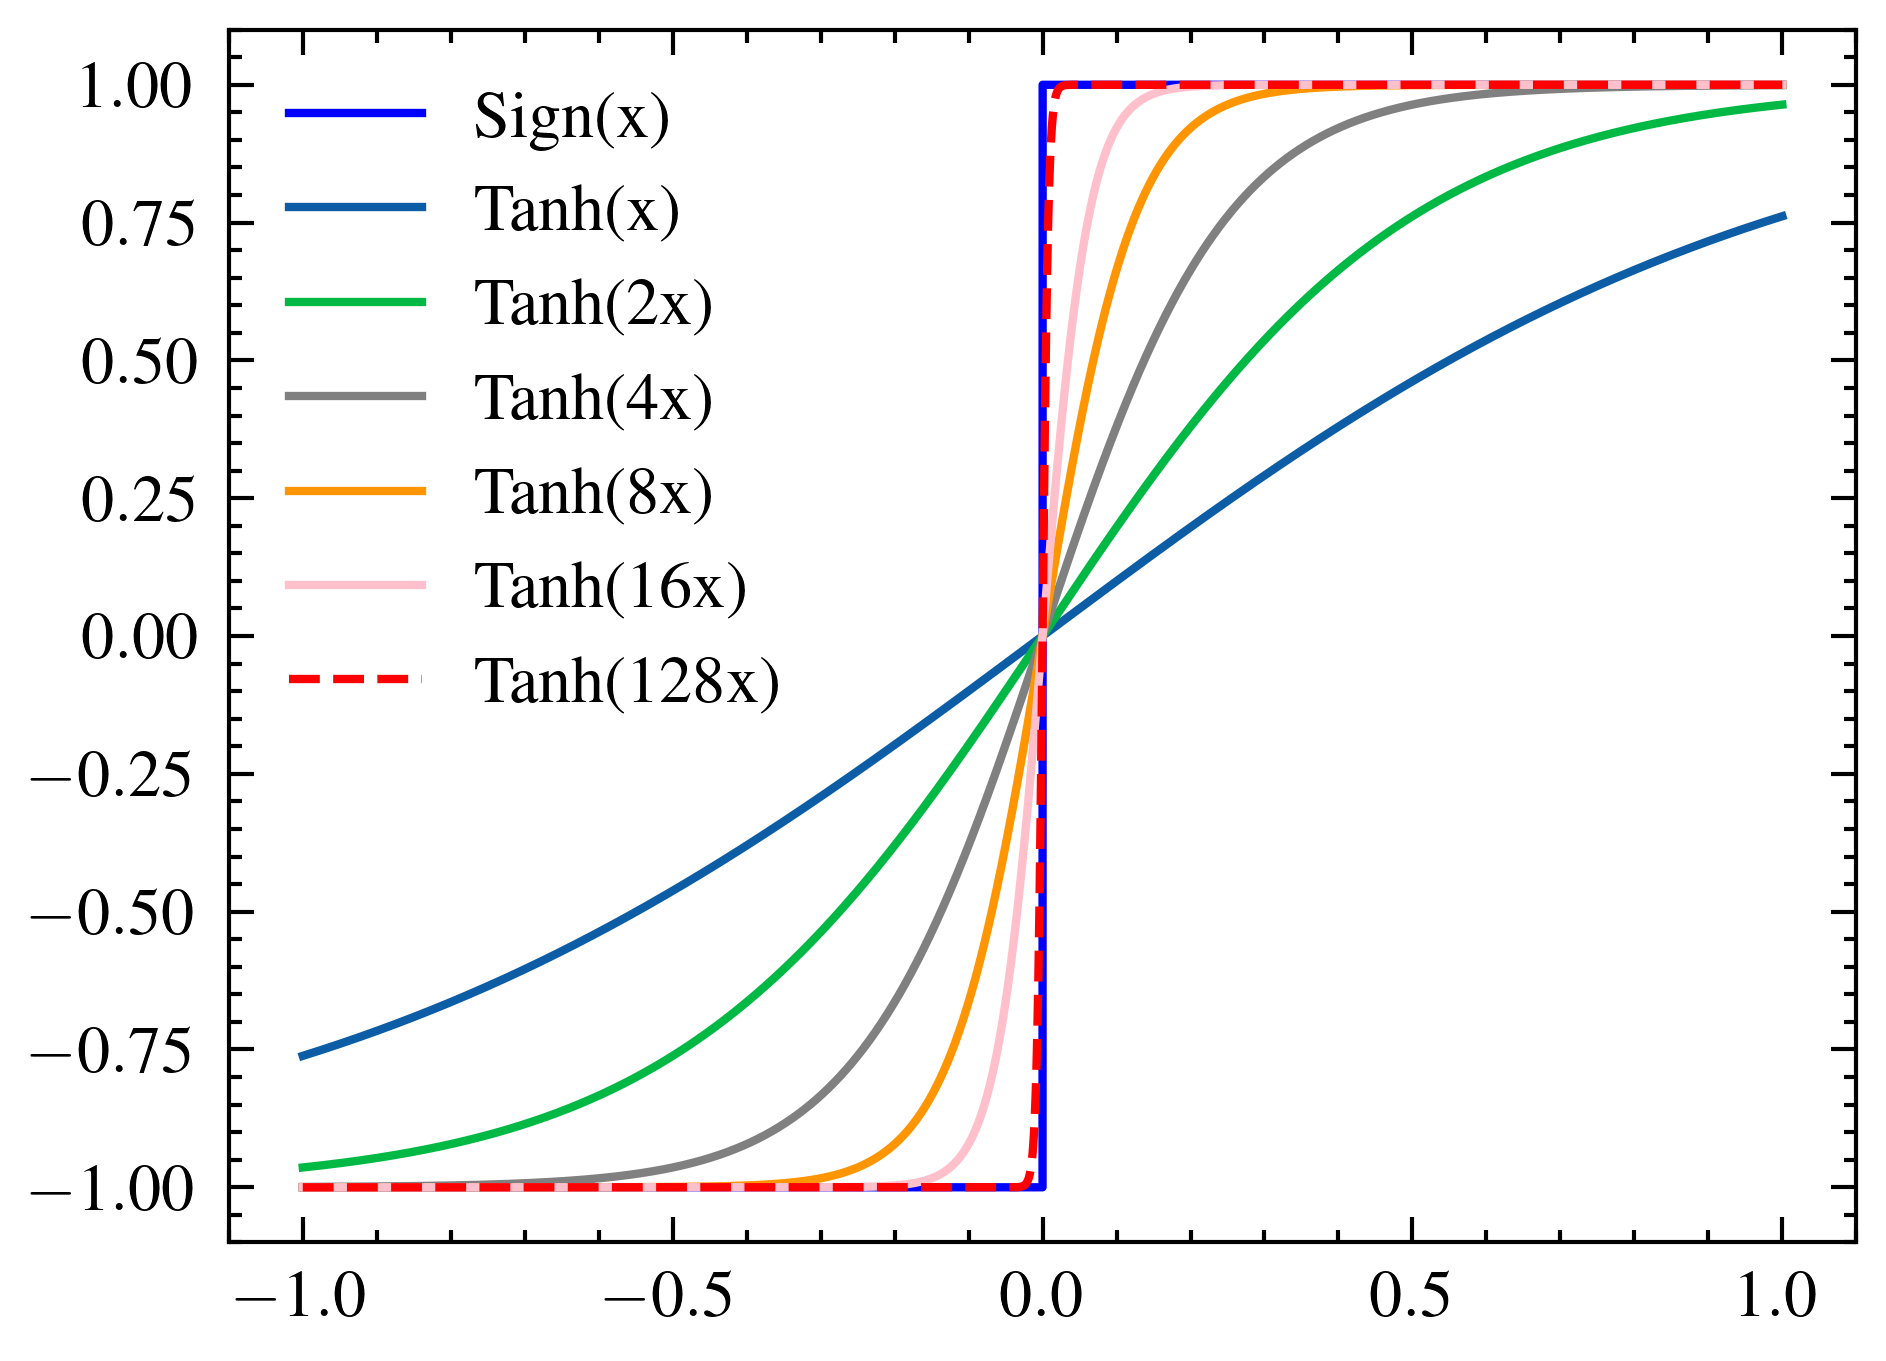
\includegraphics[width=\textwidth]{iacrtrans-0.93/figures/Sign_plot.png}
    \captionof{\textbf{a)} }{Sign and its function approximation using plain Tanh over different domains.}
    \end{minipage}
    \hfill
    \begin{minipage}{.48\textwidth}
    \centering
    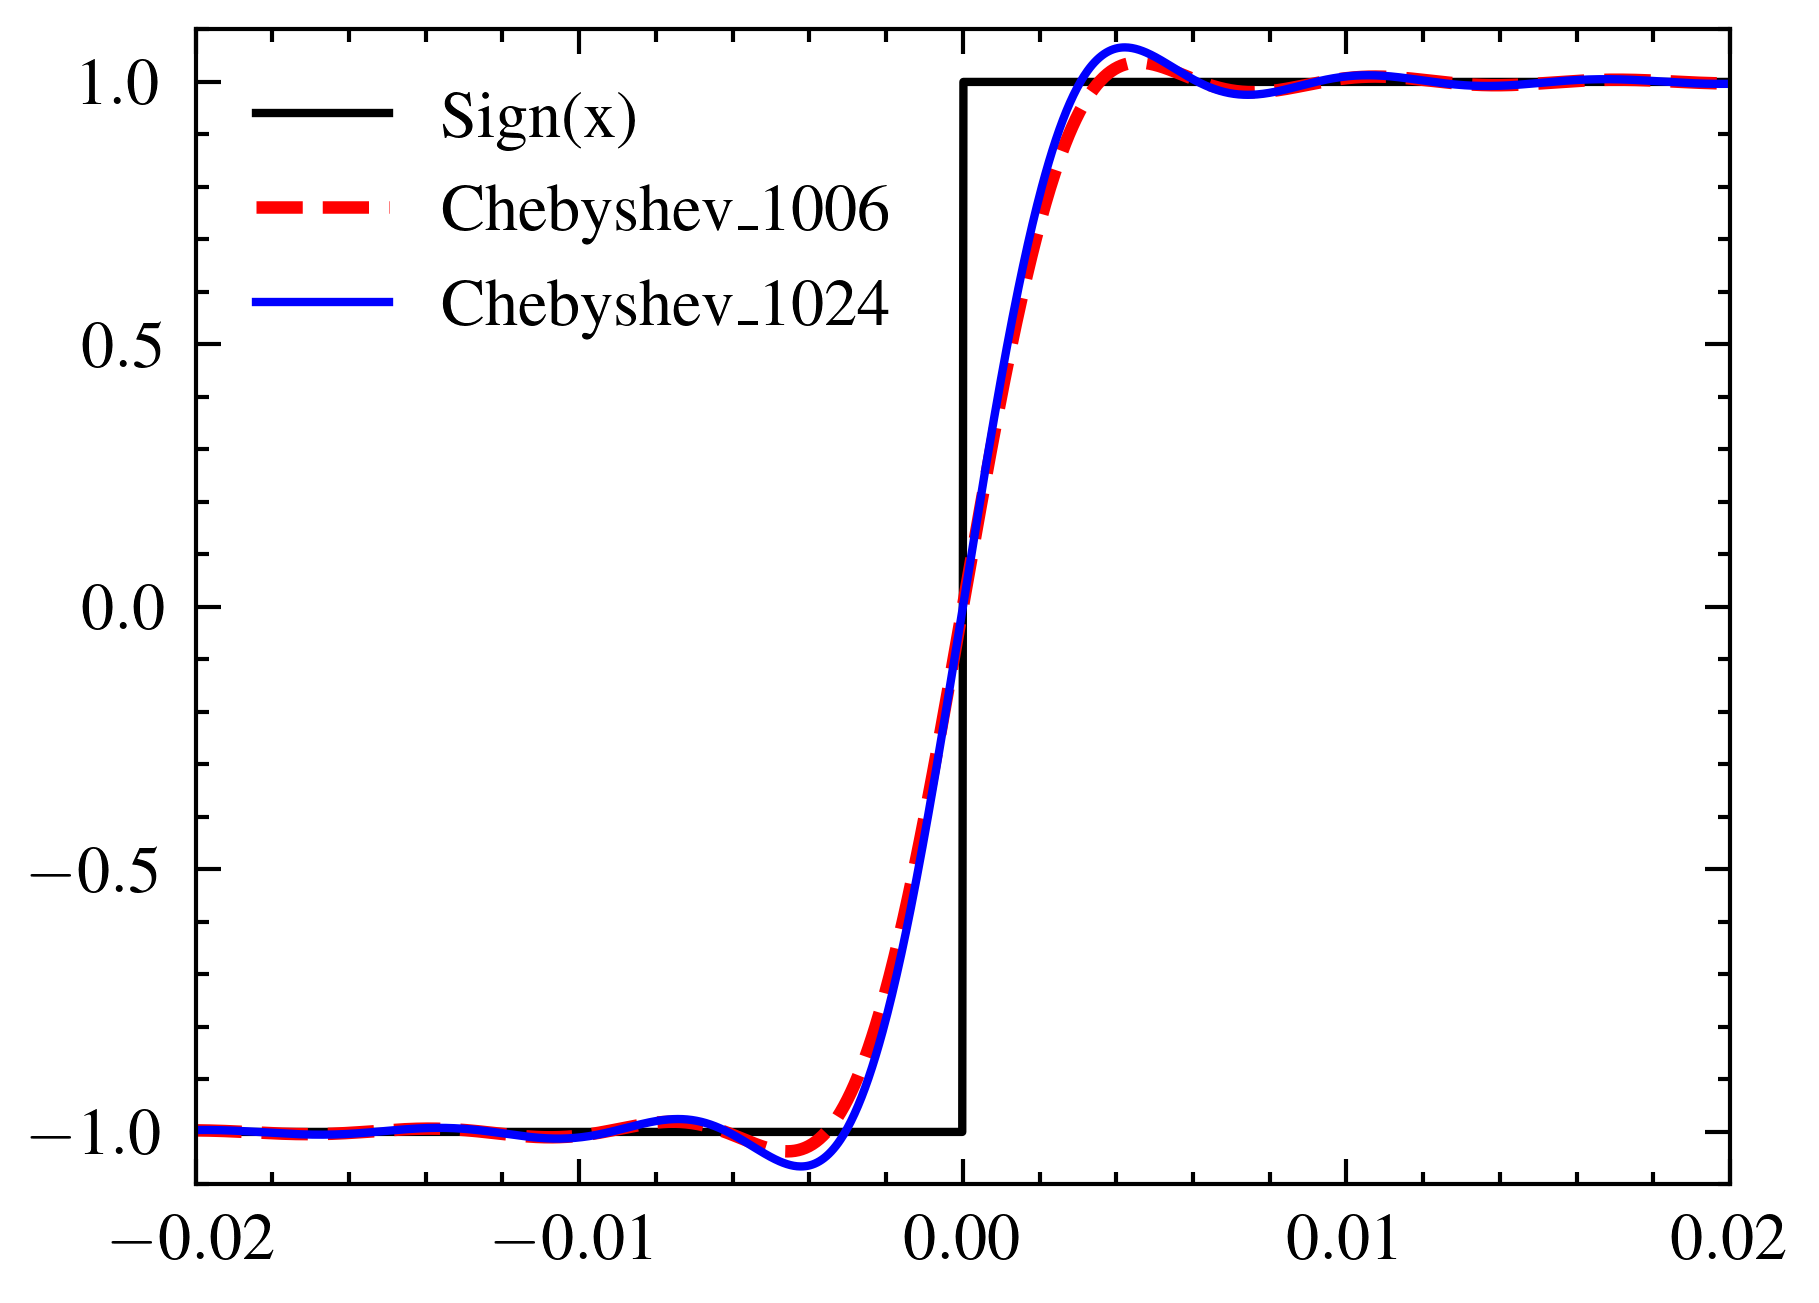
\includegraphics[width=\textwidth]{iacrtrans-0.93/figures/cheb_approx.png}
    \captionof{\textbf{b)} }{Sign and Tanh function approximation using Chebyshev series.}
    \end{minipage}
    \caption{Function approximations for the non-continuous sign function.}
    \label{fig:sign_approx_cheb}
\end{figure}

The sign function, also known as signum, plays a crucial role in determining the sign of a value. Its significance extends to various applications in machine learning, serving as a foundational element for non-linear activation functions like the Rectified Linear Unit (ReLu) or Max Pooling. This is attributed to the ability of the sign function to facilitate comparison or max operations in the following manner:
\begin{align}
    \text{comp}(a,b) &= \frac{ \text{sign}(a-b)+1}{2}\\
    \text{max}(a,b) &= \frac{ (a+b)+(a-b) \text{sign}(a-b)}{2}
\end{align}

Fully homomoprhic encryption schemes like FHEW or TFHE can precisely compute the sign function using bootstrapping-based function evaluation, resembling a look-up table. However, in approximate or integer arithmetic schemes like CKKS, BGV, BFV, etc., the absence of table look-up capabilities makes evaluating non-linear functions challenging. Consequently, these schemes resort to function approximation for sign evaluation. For example, Figure~\ref{fig:sign_approx_cheb}a) demonstrates the effective use of Tanh with a modified domain (e.g., $x, 2\times x, \cdots, 128\times x$) to approximate the sign function. Following this, a polynomial approximation of Tanh, such as the Taylor series, is applied to further approximate the sign function.

In recent years, significant progress has been made in the field of homomorphic encryption, leading researchers to explore methods for effectively approximating the sign function. One prevalent approach involves leveraging the Chebyshev series, known for its universal applicability in approximating a broad spectrum of functions. Notably, OpenFHE has already incorporated an implementation of the Chebyshev series. This implementation is used to assess the Homomorphic modular reduction during the Bootstrapping procedure.

An optimization of the sign approximation technique was introduced in \cite{Sign_approx_comp_poly}. In this research, the authors advocate for a sign approximation approach based on polynomial composition, with Chebyshev serving as the basis polynomial. They suggest and validate the effectiveness of dividing the computation depth, denoted as $d$, into smaller segments (e.g., $(d_1,d_2)$ where $d_1+d_2=d$). The proposed methodology involves initially evaluating a function that approximates the Chebyshev series for depth $d_1$. The obtained result is then utilized as an input for the Chebyshev series of depth $d_2$. Despite the promising outcomes reported by the authors, attempts to reproduce their results on the given input domain $[-1,1]$ using the OpenFHE library were unsuccessful. Therefore, next we will delve into the process of achieving the FHERMA challenge result. 

Initially, employing a straightforward approximation of the sign function through the Chebyshev series evaluation within the OpenFHE library yields an accuracy of $99.96\%$. This accuracy is achieved with a multiplicative depth of 10. It is important to note that the Chebyshev series can only be evaluated up to the coefficient $1006$ when approximating $\text{Tanh}(x\times\texttt{RAND\_MAX})$ using OpenFHE. The resulting approximation is illustrated in Figure~\ref{fig:sign_approx_cheb}b). To enhance the computational capabilities of OpenFHE, we conducted an analysis to determine the feasibility of evaluating additional Chebyshev series. Notably, since the sign function is an odd function, the even degree coefficients ($\textbf{T}_{2i}$) do not contribute to its approximation. Consequently, there is no need to evaluate these even terms of the Chebyshev series.

Building on this observation, we explored the possibility of evaluating odd degree coefficients, such as $\textbf{T}_{1009}$. In simpler terms, our objective was to establish whether it is possible to evaluate $c \times\textbf{T}_{1009}$ while adhering to the multiplicative depth limitation of 10, where $c$ is the coefficient resulting from the function approximation. We utilize the properties of the Chebyshev series and write down recursive relations as follows:

\begin{align}
    \text{c}\times\textbs{T}_{1009} && \rightarrow && \text{2c}\times\textbs{T}_{512}\times\textbs{T}_{497}-\text{c}\times\textbs{T}_{15} && \rightarrow &&  \textbs{T}_{512}\times(\text{2c}\times\textbs{T}_{497})-\text{c}\times\textbs{T}_{15}\\
    \text{2c}\times\textbs{T}_{497} && \rightarrow &&  \text{4c}\times\textbs{T}_{256}\times\textbs{T}_{241}-\text{2c}\times\textbs{T}_{15} && \rightarrow  && \textbs{T}_{256}\times(\text{4c}\times\textbs{T}_{241})-\text{2c}\times\textbs{T}_{15}\\
    \text{4c}\times\textbs{T}_{241} && \rightarrow  && \text{8c}\times\textbs{T}_{128}\times\textbs{T}_{113}-\text{4c}\times\textbs{T}_{15} && \rightarrow &&  \textbs{T}_{128}\times(\text{8c}\times\textbs{T}_{113})-\text{4c}\times\textbs{T}_{15}\\
    \text{8c}\times\textbs{T}_{113} && \rightarrow &&  \text{16c}\times\textbs{T}_{64}\times\textbs{T}_{49}-\text{8c}\times\textbs{T}_{15} && \rightarrow &&  \textbs{T}_{64}\times(\text{16c}\times\textbs{T}_{49})-\text{8c}\times\textbs{T}_{15}\\
    \text{16c}\times\textbs{T}_{49} && \rightarrow &&  \text{32c}\times\textbs{T}_{32}\times\textbs{T}_{17}-\text{16c}\times\textbs{T}_{15} && \rightarrow &&  \textbs{T}_{32}\times(\text{32c}\times\textbs{T}_{17})-\text{16c}\times\textbs{T}_{15}\\
    \text{32c}\times\textbs{T}_{17} && \rightarrow &&  \text{64c}\times\textbs{T}_{16}\times\textbs{T}_{1}-\text{32c}\times\textbs{T}_{15} && \rightarrow &&  \textbs{T}_{16}\times(\text{64c}\times\textbs{T}_{1})-\text{32c}\times\textbs{T}_{15}
\end{align}


Upon the initial breakdown of $\textbf{T}_{1009}$, we observed that the series terms to be multiplied ($\textbf{T}_{512}$, $\textbf{T}_{497}$) were at the same depth of nine. Unfortunately, this configuration made it impossible to perform a third multiplication with the coefficient $\text{c}$. Therefore, we iteratively broke down the expression until we achieved multiplicative terms at different depths. In the final equation, $\textbf{T}_{16}$ is at a depth of four, while $\textbf{T}_{1}$ is at depth 0, representing the original input ciphertext. At this stage, we can multiply $\text{c}$ with $\textbf{T}_{1}$, bringing it to a depth of one. Subsequently, we can proceed to compute upwards the recursive breakdown to obtain $c \times \textbf{T}_{1009}$. This strategy enables us to evaluate more Chebyshev series coefficients effectively.

The same methodology is applied to evaluate all the remaining Chebyshev series coefficients - $\textbf{T}_{1011}$, $\textbf{T}_{1013}$, $\textbf{T}_{1015}$, $\textbf{T}_{1017}$, $\textbf{T}_{1019}$, $\textbf{T}_{1021}$, and $\textbf{T}_{1023}$. It is crucial to note that the recursion must be further broken down to evaluate higher degree coefficients. This additional evaluation contributes to an increased accuracy from $99.96\%$ to $99.97\%$. The approximation for this is shown in the Figure~\ref{fig:sign_approx_cheb}b). With this, we conclude the FHERMA challenge solution for the SIGN problem. The newfound capability to evaluate the full depth presents an intriguing opportunity to explore potential improvements or attempt to reproduce the results outlined in~\cite{Sign_approx_comp_poly}. This increased depth computation also serves to improve the efficiency of other function approximations, for example, the logistic function.

\subsection{Matrix Multiplication}

Matrix multiplication is a crucial aspect of advanced mathematics and plays a central role in machine learning, especially in Neural Networks (NN). Certain components of a network, like fully connected layers or filter/kernel, rely on efficient matrix multiplication. Though there are efficient algorithms like Strassen's algorithm for plaintext operations, conducting matrix multiplication in an encrypted domain is a newer research area. This has gained attention because it enables encrypted machine learning training or inference using fully homomorphic encryption schemes like CKKS, which can handle approximate arithmetic.

Encrypted matrix multiplication techniques in literature can be broadly categorized into three types. The first type involves a depth of two multiplications and utilizes a simple row-wise encoding. An example is the work cited as \cite{mult2_d2}, which presents a general technique. For a square matrix with dimensions $d\times d$, this method requires only $2 d+3\log_2(d)-2$ rotations and $2d$ multiplications. It is important to note that these two operations are the most costly, as an expensive key-switch operation is needed after each one to ensure the ciphertext remains decryptable using the same secret key. A drawback of this approach is the necessity for $d^3$ slots packing availability in the ciphertext. Hence, it does not scale well for big matrices.

The second category of techniques, as described in \cite{mult1_d3}, deviates slightly from previous methods by using diagonal-based matrix multiplication. Although this technique requires $3d+5\sqrt{d}$ rotations and $4d$ multiplications initially, with increased packing, it can be optimized to only need $d+2\sqrt{d}$ computations. However, a significant drawback is the requirement for three multiplicative depths. While the algorithms proposed in \cite{mult1_d3} can be modified to operate within a multiplicative depth of two, doing so results in a much more significant increase in the number of rotations and multiplications.

The third and final category of works, as presented in \cite{mult1_d2_pc, mult2_d2_pc, mult3_d2_pc}, significantly deviates from the previous two types. These works aim to leverage a multivariate variant of the CKKS scheme (m-RLWE)~\cite{mheaan}, enabling the encoding of a matrix into a hypercube structure. This approach facilitates cost-effective row-wise and column-wise rotations, optimizing matrix multiplication while only requiring a multiplicative depth of two. However, note that the multivariate CKKS is incompatible with the original CKKS. Additionally, the parameters of the multivariate CKKS are not standardized, and its initial proposal~\cite{mrlwe} was found to be insecure \cite{mrlwe_attack}.



\begin{algorithm}
    \renewcommand{\algorithmicensure}{\textbf{Out:}}
    \caption{$\mathtt{Matrix.Mult}$ (1 Matrix packing version of \cite{mult2_d2}) }
    \begin{algorithmic}[1]
        \Require $A,B \gets \text{row\_enc}(\mathtt{A}_{d\times d},\mathtt{B}_{d\times d})$
        \Ensure  $C=\text{row\_enc}(\mathtt{A}_{d\times d}\times\mathtt{B}_{d\times d})$ 
        \Statex \LeftComment{\textcolor{gray}{// Preprocess $A$ }}
        \For{$j=0$ to $d-1$}	
        \State $\tilde{A}[j] \gets  \texttt{cMult}(A, \pi_{j} )$ \Comment{\textcolor{gray}{Splitting $A$ column-wise}}
        \State $\tilde{A}[j] \gets  \texttt{Rot}(\tilde{A}[j],-j)$ \Comment{\textcolor{gray}{ Right align all the columns}}
        
        \For{$i=0$ to $\log_2(d)-1$}	\Comment{\textcolor{gray}{ Replicate the column}}
        \State $\tilde{A}[j] +=  \texttt{Rot}(\tilde{A}[j], -(2^i) )$
     \EndFor
     \EndFor
     \Statex \LeftComment{\textcolor{gray}{// Preprocess $B$ }}
        \For{$j=0$ to $d-1$}	
        \State $\tilde{B}[j] \gets  \texttt{cMult}(B, \psi_{j} )$ \Comment{\textcolor{gray}{ Splitting $B$ row-wise}}
        \State $\tilde{B}[j] \gets  \texttt{Rot}(\tilde{B}[j],-j*d)$ \Comment{\textcolor{gray}{Top align all the rows}}
        \For{$i=0$ to $\log_2(d)-1$}	\Comment{\textcolor{gray}{ Replicate the rows}}
        \State $\tilde{B}[j] +=  \texttt{Rot}(\tilde{B}[j], -(2^i)*d )$
     \EndFor
     \EndFor
     \Statex \LeftComment{\textcolor{gray}{// Compute $C$ }}
        \For{$j=0$ to $d-1$}	
        \State $C += \texttt{cMult}(\tilde{A}[j],\tilde{B}[j] )$ 
     \EndFor
    \end{algorithmic}\label{algo:mult_1}
    \end{algorithm}

Due to the FHERMA challenge restrictions, which limit the multiplicative depth to two and ciphertext encoding to row-wise, applying techniques like the one in \cite{mult2_d2} directly is not feasible when the available slots ($n=8192$) do not meet the requirement of $d^3$ slots for a given dimension of $d=64$. Therefore, we first explore adapting the technique from \cite{mult2_d2} to our case. The adapted technique is outlined in Algorithm~\ref{algo:mult_1}, which utilizes column and row masks ($\pi_i$ and $\psi_i$, respectively). The complexity of this adaptation is $2d+d\log_2{d}-1$ rotations and $3d$ multiplications. Since it is possible to pack two matrices into one ciphertext, the algorithm can be optimized to consume $2d+d\log_2{d}-1$ rotations and $\frac{5d}{2}$ multiplications. This optimization is achieved by aligning rotations at Steps 3 and 8 and then packing two ciphertexts.

To further optimize the current literature's best attempt at a multiplicative depth two matrix multiplication, we explore a strategy involving the initial packing of duplicates of the same ciphertext (one original and one rotated). This optimization leads to a significant reduction in the number of rotations. The proposed Algorithm~\ref{algo:mult_2} outlines this approach, where both ciphertexts $A$ and $B$ undergo pre-processing. Following this packing strategy, only $d\log_2{d}+1$ rotations and $\frac{3d}{2}$ multiplications are required for the subsequent steps.
\begin{algorithm}
    \renewcommand{\algorithmicensure}{\textbf{Out:}}
    \caption{$\mathtt{Optimized.Matrix.Mult}$ }
    \begin{algorithmic}[1]
        \Require $A,B \gets \text{row\_enc}(\mathtt{A}_{d\times d},\mathtt{B}_{d\times d})$
        \Ensure  $C=\text{row\_enc}(\mathtt{A}_{d\times d}\times\mathtt{B}_{d\times d})$ 
        \Statex \LeftComment{\textcolor{gray}{// Preprocess $A$ }}
        \State $A +=  \texttt{Rot}(A, -d*d+1 )$
        \For{$j=0$ to $(d/2)-1$}	
        \State $\tilde{A}[j] \gets  \texttt{cMult}(A, \pi_{j,j+d*d} )$ \Comment{\textcolor{gray}{Splitting $A$ column-wise}}
        \State $\tilde{A}[j] \gets  \texttt{Rot}(\tilde{A}[j],-2j)$ \Comment{\textcolor{gray}{ Right align all the columns}}
        
        \For{$i=0$ to $\log_2(d)-1$}	\Comment{\textcolor{gray}{ Replicate the column}}
        \State $\tilde{A}[j] +=  \texttt{Rot}(\tilde{A}[j], -(2^i) )$
     \EndFor
     \EndFor
     \Statex \LeftComment{\textcolor{gray}{// Preprocess $B$ }}
     \State $B +=  \texttt{Rot}(B, -d*d+d )$
        \For{$j=0$ to $(d/2)-1$}	
        \State $\tilde{B}[j] \gets  \texttt{cMult}(B, \psi_{j,j+d*d} )$ \Comment{\textcolor{gray}{ Splitting $B$ row-wise}}
        \State $\tilde{B}[j] \gets  \texttt{Rot}(\tilde{B}[j],-2j*d)$ \Comment{\textcolor{gray}{Top align all the rows}}
        \For{$i=0$ to $\log_2(d)-1$}	\Comment{\textcolor{gray}{ Replicate the rows}}
        \State $\tilde{B}[j] +=  \texttt{Rot}(\tilde{B}[j], -(2^i)*d )$
     \EndFor
     \EndFor
     \Statex \LeftComment{\textcolor{gray}{// Compute $C$ }}
        \For{$j=0$ to $(d/2)-1$}	
        \State $C += \texttt{cMult}(\tilde{A}[j],\tilde{B}[j] )$ 
     \EndFor
     \State $C += \texttt{Rot}(c,d* d )$
    \end{algorithmic}\label{algo:mult_2}
    \end{algorithm}

Additionally, this algorithm exhibits high parallelizability. Hence, employing `\textit{pragma omp parallel}' before the for loops can help leverage the capabilities of modern multithreaded operating systems, leading to excellent performance. It is important to highlight that the proposed approach is tailored to the constraints of the FHERMA challenge, considering the available packing $2d^2$ and matrix dimension $d$. Notably, the scalability of this approach improves with higher packing availability. It outperforms existing methods like \cite{mult2_d2, mult1_d3} by consuming only $\mathcal{O}(\log_2{d})$ rotations while still requiring a multiplicative depth of two. The proposed algorithm is characterized by its simplicity, yet it achieves non-trivial results, particularly when applied to higher packing scenarios. Its effectiveness lies in its ability to provide favourable outcomes under these conditions.

Extending and applying the proposed approach to rectangular matrices and scenarios involving smaller matrix filters applied to a matrix present intriguing possibilities for future exploration. Generalizing the algorithm to handle different matrix shapes and sizes could enhance its versatility and applicability in various contexts within the field of encrypted matrix multiplication.
\end{document}